\section{Obiettivi e apparato sperimentale}
In questo esperimento si vuole verificare la legge di Coulomb, analizzando la dipendenza della forza elettrostatica dalla distanza e dalla carica elettrica mediante una bilancia di torsione, secondo la seguente relazione:

\begin{equation}
    F_C = \frac{1}{4\pi \varepsilon_0 \varepsilon_r} \cdot \frac{q_1 q_2}{r^2}
    \label{Coulomb}
\end{equation}

Una volta misurata la costante di torsione del filo, sfruttando la legge del momento torcente, sarà possibile ottenere la costante dielettrica $\varepsilon_{0}$ del vuoto e confrontarla col valore atteso di $8.85\cdot10^{-12}$ $\text{C}^2/\text{Nm}^2$.

\begin{figure}[H]
    \centering
    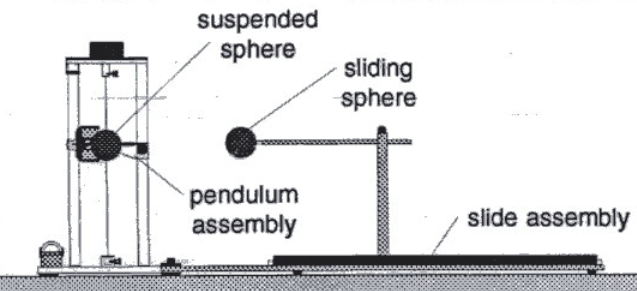
\includegraphics[width=0.8\textwidth]{Immagini/App.png}
    \caption{Apparato sperimentale: bilancia di torsione.} 
    \label{fig:Apparato}
\end{figure}

Come mostrato in Figura 1, una sfera leggera, ricoperta di vernice conduttiva, è sostenuta da un braccio rigidamente collegato ad un equipaggio mobile, contrappesato, ancorato a sua volta ad un sottile filo di torsione. La sfera può ruotare torcendo il filo. Una sfera identica è montata su un supporto a slitta, in modo che si possa posizionare a diverse distanze rispetto la prima.
Tramite un elettrodo collegato al generatore di alta tensione, si caricano entrambe le sfere con carica dello stesso segno: la forza
elettrostatica fra le due sfere causa l'allontanamento della sfera mobile che, essendo vincolata al filo, si allontana ruotando di un certo angolo: ruotando la testa di sospensione del filo in senso contrario, si riporta l'equipaggio mobile nella posizione di equilibrio iniziale e si misura l'angolo di torsione. All'equilibrio, il momento della forza elettrostatica è uguale al momento elastico sviluppato dal filo, ne segue:

\begin{equation}
    \tau_{Coulomb} = F_C \cdot b = C_{\text{tor}} \cdot \theta = \tau_{tor}
    \label{eq:Momento}
\end{equation}
    
\newpage

\section{Dipendenza di \boldmath $F_C$ dalla distanza}
Si vuole verificare la dipendenza della forza di Coulomb dall'inverso del quadrato della distanza tra le cariche: dalle relazioni \eqref{Coulomb} e \eqref{eq:Momento} segue che l'angolo di torsione $\theta$ risulta direttamente proporzionale alla forza applicata, ergo si può studiare la sua dipendenza dalla distanza r tra i centri delle sfere.

Si allontanano le due sfere alla massima distanza possibile e si caricano entrambe ad un potenziale di 6 kV tramite una sonda di carica. Il diametro delle sfere, d = $(3.9 \pm 0.1)$ cm, è stato misurato mediante calibro. Si procede portando la sfera mobile alla prima distanza selezionata: la forza repulsiva agente fra le due sfere farà ruotare l'equipaggio mobile appeso al filo di torsione. Si prosegue ruotando in verso opposto la manopola di azzeramento della torsione del filo, fino a far coincidere lo zero dell'equipaggio mobile con quello fisso. Si ripete il procedimento per valori  crescenti di r, raccogliendo i valori di $\theta$: le misure effettuate sono riportati in Tabella 1. 

\begin{table}[H]
\centering
\begin{tabular}{l l *{5}{S[table-format=3.2, table-number-alignment=center]}} 
\toprule
& & {\textbf{10cm}} & {\textbf{12cm}} & {\textbf{14cm}} & {\textbf{19cm}} & {\textbf{22cm}} \\
\midrule
& & 97.0 & 70.0 & 49.0 & 28.0 & 20.0 \\
& & 101.0 & 68.0 & 51.0 & 28.0 & 18.0 \\
& & 99.0 & 71.0 & 53.0 & 31.0 & 22.0 \\
\midrule
{\textbf{\boldmath$\bar{\theta}$}}         & {(\text{°})}    & 99.0 & 69.7 & 51.0 & 29.0 & 10.0 \\
{\textbf{\boldmath$\sigma_{\theta}$}}      & {(\text{°})}    & 2.0  & 1.5 & 2.0 & 1.7 & 2.0 \\
{\textbf{\boldmath$\bar{\sigma}_{\theta}$}} & {(\text{°})}    & 1.2  & 0.9 & 1.2 & 1.0 & 1.2 \\
\midrule
{\textbf{\boldmath$\bar{\theta}$}}         & {(\text{rad})}    & 1.73 & 1.22 & 0.89 & 0.51 & 0.35 \\
{\textbf{\boldmath$\sigma_{\theta}$}}      & {(\text{rad})}    & 0.03  & 0.03 & 0.03 & 0.03 & 0.03 \\
{\textbf{\boldmath$\bar{\sigma}_{\theta}$}} & {(\text{rad})}    & 0.02  & 0.02 & 0.02 & 0.02 & 0.02 \\
\bottomrule
\end{tabular}
\caption{Angoli di torsione e loro valore medio, incertezza ed errore standard della media in funzione di r, distanza tra i centri delle sfere.}
\label{tab:distanza}
\end{table}

Le cariche sono libere di muoversi sulla superficie della sfera e, in assenza di forze elettrostatiche esterne, la loro distribuzione è uniforme sull'intera superficie: in queste condizioni, la sfera conduttrice carica si può approssimare ad una carica puntiforme posta nel centro della sfera. Tuttavia, quando le due sfere cariche sono vicine, le cariche mobili si ridistribuiscono in modo da rendere minima l'energia elettrostatica, posizionandosi il più lontano possibile da quelle della sfera opposta. 
La distanza reale tra le cariche è quindi maggiore di quella tra i centri delle sfere, dunque la forza di Coulomb diminuisce. Questo effetto è particolarmente significativo quando la distanza tra le sfere è confrontabile con il loro raggio e dunque per tali valori la dipendenza lineare non è ben verificata.
\newpage
Si corregge la relazione tra l'angolo $\theta$ e la distanza moltiplicando il valore dell'angolo per un fattore 1/B, con:

\begin{equation}
    B(r)=1-\frac{4a^3}{r^3}
    \label{1}
\end{equation}

dove $a$ è il raggio delle sfere ed $r$ è la distanza tra i loro centri. Si procede con l'interpolazione dei valori di $\theta$ corretti in funzione di $1/r^2$ determinando la miglior retta che descrive la relazione, come mostrato in Figura 2.

\begin{figure}[H]
    \centering
    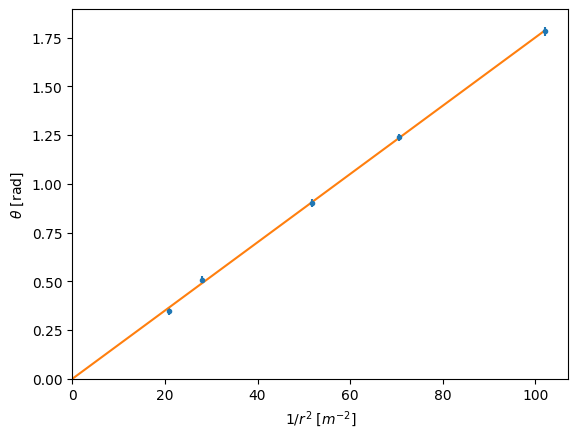
\includegraphics[width=0.6\textwidth]{Immagini/Distanza.png}
    \caption{Interpolazione lineare di $\theta$ corretto in funzione di $1/r^2$, imponendo il passaggio per l'origine.} 
    \label{fig:Distanza}
\end{figure}

Il coefficiente angolare della retta interpolata è $k_1=(17.5 \pm 0.1) \cdot10^{-3}\: \text{m}^{2}$. Il test del $\chi^2$ della retta è $\tilde{\chi_o}^2= 0.44$, che per 4 gradi di libertà restituisce una probabilità di accordo con i dati del $78\%$.

\section{Dipendenza di \boldmath $F_C$ dalla carica}
\subsection{Potenziale Uguale}
Per determinare la dipendenza della forza di Coulomb dalla carica è necessario eseguire misure nelle stesse modalità precedenti, mantenendo però fissa la distanza tra le due sfere: le misure sono state effettuate ad una distanza di $(12.0 \pm 0.1)$ cm. 
A piccole distanze la capacità delle sfere è circa costante, ed essendo la carica direttamente proporzionale al potenziale, secondo la relazione $q = C\cdot V$, dove $C=4\pi \varepsilon_{0} a$ è la capacità di una sfera isolata, è sufficiente studiare, tramite le relazioni \eqref{Coulomb} e \eqref{eq:Momento}, la dipendenza della forza dal potenziale.
\newpage

Si caricano le sfere allo stesso potenziale, in valori crescenti fino a 6 kV. Per il potenziale si è stimato un errore dell'1\%, tenendo in considerazione inevitabili dispersioni di carica. Per gli angoli, l'incertezza di 4° è dovuta ad una combinazione di possibili errori sistematici di azzeramento della strumentazione, di sensibilità ed oscillazioni residue. Le misure sono state raccolte in tabella 2.

\begin{table}[H]
\centering
\begin{tabular}{S[table-format=4.0] S[table-format=2.0] S[table-format=2.0] S[table-format=1.2] S[table-format=1.2]} 
\toprule
{\textbf{Potenziale}} & {\textbf{\boldmath$\sigma_V$}} & {\textbf{\boldmath$\theta$}} & {\textbf{\boldmath$\theta$}} & {\textbf{\boldmath$\sigma_\theta$}} \\
{\text{(V)}}  & {\text{(V)}}  & {\text{(°)}} & {\text{(rad)}} & {\text{(rad)}} \\
\midrule
2000 & 60 & 10 & 0.17 & 0.07 \\
2500 & 60 & 14 & 0.24 & 0.07 \\
3000 & 60 & 20 & 0.35 & 0.07 \\
3500 & 60 & 23 & 0.40 & 0.07 \\
4000 & 60 & 35 & 0.61 & 0.07 \\
4500 & 60 & 41 & 0.72 & 0.07 \\
5000 & 60 & 48 & 0.84 & 0.07 \\
5500 & 60 & 62 & 1.08 & 0.07 \\
6000 & 60 & 70 & 1.22 & 0.07 \\
\bottomrule
\end{tabular}
\caption{Potenziale, angoli di torsione e relativa incertezza.}
\label{tab:potenziale_uguale}
\end{table}

Si interpolano linearmente gli angoli di torsione in funzione del potenziale $V^2$, applicando agli angoli la correzione 1/B, come in Figura 3.

\begin{figure}[H]
    \centering
    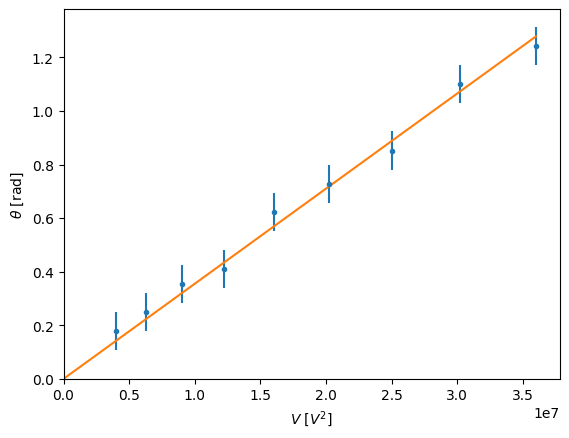
\includegraphics[width=0.65\textwidth]{Immagini/PotUguale.png}
    \caption{Interpolazione lineare di $\theta$ corretto in funzione di $V^2$, imponendo il passaggio per l'origine.} 
    \label{fig:PotUguale}
\end{figure}

Il coefficiente angolare della retta interpolata è $k_2=(35 \pm 1)\: \text{nV}^{2}$. Il test di adattamento del $\chi^2$ restituisce un $\tilde{\chi_o}^2= 0.25$, che per 8 gradi di libertà corrisponde ad una probabilità di accordo con i dati del $98\%$.
\newpage

\subsection{Potenziale Diverso}
Si ripetono le misure mantenendo costante il potenziale su una sfera e variandolo sull'altra. È stato considerato un potenziale fisso pari a 6 kV, mentre gli errori sono stati stimati come in Tabella 2. In Tabella 3 sono riportati i valori misurati.

\begin{table}[H]
\centering
\begin{tabular}{S[table-format=4.0] S[table-format=2.0] S[table-format=2.0] S[table-format=1.2] S[table-format=1.2]} 
\toprule
{\textbf{Potenziale}} & {\textbf{\boldmath$\sigma_V$}} & {\textbf{\boldmath$\theta$}} & {\textbf{\boldmath$\theta$}} & {\textbf{\boldmath$\sigma_\theta$}} \\
{\text{(V)}}  & {\text{(V)}}  & {\text{(°)}} & {\text{(rad)}} & {\text{(rad)}} \\
\midrule
2000 & 60 & 28 & 0.49 & 0.07 \\
2500 & 60 & 35 & 0.61 & 0.07 \\
3000 & 60 & 39 & 0.68 & 0.07 \\
3000 & 60 & 39 & 0.68 & 0.07 \\
3500 & 60 & 43 & 0.75 & 0.07 \\
4000 & 60 & 52 & 0.91 & 0.07 \\
4500 & 60 & 59 & 1.03 & 0.07 \\
5000 & 60 & 61 & 1.06 & 0.07 \\
5500 & 60 & 65 & 1.13 & 0.07 \\
6000 & 60 & 70 & 1.22 & 0.07 \\
\bottomrule
\end{tabular}
\caption{Potenziale, angoli di torsione e relative incertezze.}
\label{tab:potenziali_diversi}
\end{table}

Si procede ad interpolare gli angoli di torsione in funzione del potenziale variabile, ricordandosi la correzione 1/B, assumendo un parametro libero come mostrato in Figura 4.

\begin{figure}[H]
    \centering
    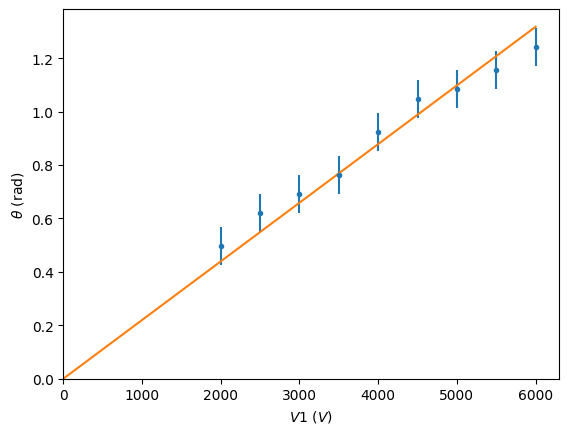
\includegraphics[width=0.6\textwidth]{Immagini/PotDiverso.png}
    \caption{Interpolazione lineare di $\theta$ corretto in funzione di $V$, imponendo il passaggio per l'origine.} 
    \label{fig:PotDiverso}
\end{figure}

La retta ha coefficiente angolare $k_3=(220 \pm 6)$ $\mu \text{V}$. Il test del $\chi^2$ per il modello lineare restituisce un $\tilde{\chi_o}^2= 0.59$, che per 8 gradi di libertà corrisponde ad una probabilità di accordo con i dati del $78\%$.

\section{Misura della costante di torsione del filo}
Per determinare la costante $C_{\text{tor}}/b$ si deve calibrare la bilancia di torsione utilizzando una forza nota che agisca sulla sfera mobile al posto della forza di Coulomb: si utilizza la forza di gravità. Si colloca la bilancia sul fianco e si posiziona un tubo di supporto sotto la sfera, per sostenerla fino a calibrazione ultimata ed evitare torsioni eccessive del filo.
Si azzera la bilancia, ruotando la manopola di regolazione della torsione, fino a portare l'indice inciso sul contrappeso a paletta in corrispondenza di quello segnato sul braccio fisso: all'equilibrio, la bacchetta di sostegno della sfera mobile deve risultare perfettamente orizzontale.
Si prosegue appoggiando cautamente masse di valore crescente sulla sfera mobile, per poi regolare la manopola della torsione fino a riportare la sfera nella posizione di equilibrio di partenza. L'incertezza sugli angoli è stata stimata come nelle sezioni precedenti: le misure sono riportate in Tabella 4.

\begin{table}[H]
\centering
\begin{tabular}{S[table-format=2.0] S[table-format=3.0] S[table-format=1.2] S[table-format=1.2]} 
\toprule
{\textbf{m (mg)}} & {\textbf{\boldmath$\theta$ (°)}} & {\textbf{\boldmath$\theta$ (rad)}} & {\textbf{\boldmath$\sigma_\theta$ (rad)}} \\
\midrule
20 & 136 &  2.37 & 0.07 \\
40 & 282 &  4.92 & 0.07 \\
50 & 355 &  6.20 & 0.07 \\
70 & 500 &  8.73 & 0.07 \\
90 & 645 & 11.26 & 0.07 \\
\bottomrule
\end{tabular}
\caption{Massa, angoli di torsione e relative incertezze.}
\label{tab:costante:torsione}
\end{table}

All'equilibrio si possono eguagliare i momenti della forza di gravità $F_G$ e di quella di torsione, e si ha $F_G \cdot b = m\cdot g \cdot b = C_{\text{tor}} \cdot \theta$,
dove b è il braccio della forza e $C_{\text{tor}}$ la costante di torsione del filo.
Una volta definito  $K_{\text{tor}} = C_{\text{tor}}/b$, si ottiene $m\cdot g = K_{\text{tor}}\cdot \theta$: si interpolano linearmente i valori delle masse in funzione degli angoli di torsione, come in Figura 5.

\begin{figure}[H]
    \centering
    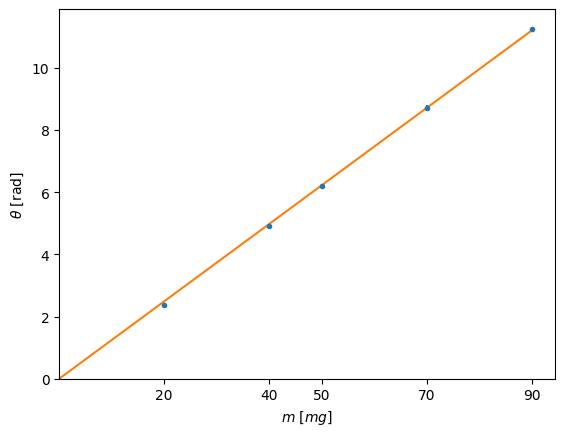
\includegraphics[width=0.6\textwidth]{Immagini/Torsione.png}
    \caption{Interpolazione lineare di $\theta$ in funzione di $m$, avendo imposto il passaggio per l'origine.} 
    \label{fig:Torsione}
\end{figure}

Dividendo $g$ per il coefficiente angolare interpolato si ottiene $K_{\text{tor}} = (78.8 \pm 0.3)$ $\mu\text{N}$. Il test del $\chi^2$ per il modello lineare restituisce $\tilde{\chi_o}^2= 1.06$, che per 4 gradi di libertà indica una probabilità di accordo con i dati del $38\%$.

\section{Misura della costante dielettrica del vuoto}
Noto il valore di $K_{\text{tor}}$, è possibile ricavare la costante dielettrica del vuoto $\varepsilon_0$, avendo approssimato $\varepsilon_r=1$ la costante dielettrica relativa dell’aria. Infatti, manipolando le equazioni \eqref{Coulomb} e \eqref{eq:Momento}, oltre alle dipendenze studiate nelle sezioni precedenti, si ottiene la seguente relazione:

\begin{equation}
    F_C = \frac{4\pi \varepsilon_0 a^2V_1V_2}{r^2} = K_{\text{tor}} \cdot \theta
\end{equation}

Dunque, a partire dai coefficienti angolari precedentemente interpolati, si calcolano i valori di $\varepsilon_0$ e se ne fa una media pesata da cui si ottiene $\bar{\varepsilon}_{0} = (8.36 \pm 0.52)\cdot10^{-12}$ $\text{C}^2/\text{Nm}^2$.

\section{Conclusioni}
L'esperienza ha permesso di effettuare tre misure indipendenti della costante dielettrica del vuoto tramite la legge di Coulomb e quella del momento di torsione, adoperata inoltre per misurare la costante di torsione del filo.
La media pesata $\bar{\varepsilon}_{0}$ delle tre misure risulta compatibile col valore previsto $\varepsilon_0 = 8.85\cdot10^{-12}$ $\text{C}^2/\text{Nm}^2$ con una probabilità del $34\%$, corrispondente a:

\begin{equation}
    t_0=\frac{\abs{\varepsilon_0-\bar{\varepsilon}_{0}}}{\sigma_{\bar{\varepsilon}_{0}}}=0.96
\end{equation}

e, infatti, il valore atteso di $\varepsilon_0$ è entro 1$\sigma_{\bar{\varepsilon}_{0}}$ da quello misurato.
\newpage